% vim: ft=tex fdm=marker et sts=2 sw=2 cole=0
%
% vitae.tex -- a minimalistic LaTeX template for resumes
%
% The design is intentionally minimalistic and I don't use
% LaTeX packages that are not part of the standard TeXLive
% distribution, and one should be able to distribute the
% entire resume as a single LaTeX file.  The styling and
% layout was partially inspired by Donald Knuth's CV [1].
%
% Copyright (c) 2014-2024, Manu Mannattil.
% All rights reserved.
%
% Usage, modification, and distribution of this document,
% for any purpose, with or without attribution, is permitted
% provided the author's personal/professional details are
% removed.
%
% [1] https://www-cs-faculty.stanford.edu/~knuth/vita.pdf
%

% Preamble {{{1
% -------------

\documentclass[10pt,a4paper,article,oneside]{memoir}

\def\fname{Manu Mannattil}                % Set your full name here.
\def\iname{M.~Mannattil}                  % Set your intials + last name here.
\def\bname{\underline{Manu Mannattil}}    % Set your name as you'd like it to appear in bibliographies.

\usepackage[T1]{fontenc}
\usepackage[utf8]{inputenc}
\usepackage{microtype}

\setlrmarginsandblock{1.25in}{1.25in}{*}
\setulmarginsandblock{1.25in}{1.25in}{*}
\checkandfixthelayout

\usepackage{color}
\definecolor{bs1}{rgb}{0.207843,0.415686,0.623529}
\definecolor{gray}{rgb}{0.5,0.5,0.5}

\usepackage[
  allcolors=bs1,
  colorlinks=true,
  pdftex,
  pdfauthor={\fname},
  pdftitle={Curriculum Vitae: \fname},
  pdfsubject={Curriculum Vitae},
  pdfkeywords={curriculum vitae, resume, vitae}
]{hyperref}
\urlstyle{same}

% Custom commands.
\def\email#1{\href{mailto:#1}{#1}}
\def\doi#1#2{\href{https://doi.org/#1}{#2}}
\def\arxiv#1#2{\href{https://arxiv.org/abs/#1}{arXiv:#1 [#2]}}

%\usepackage{mlmodern}
%\usepackage{times}
%\def\bfdefault{b}

\usepackage{mathpazo}

% Section styling.
\setsecheadstyle{\bfseries}
\setbeforesecskip{1.25\baselineskip}
\setaftersecskip{0.37\baselineskip}
\setsubsecheadstyle{\itshape}
\setbeforesubsecskip{0.75\baselineskip}
\setaftersubsecskip{0.25\baselineskip}
\setcounter{secnumdepth}{0}

\def\baselinestretch{1.0625}

% From Section 3.5 of memoir's documentation.
\clubpenalty=9996
\widowpenalty=9999
\brokenpenalty=4991
\predisplaypenalty=10000
\postdisplaypenalty=1549
\displaywidowpenalty=1602

% Hanging paragraphs throughout.
\def\hangpars{%
  \leftskip=1.75em%
  \parindent=-\leftskip%
  \setsecindent{-\leftskip}%
  \setsubsecindent{-\leftskip}%
  \parskip=0pt
}

% Reset hanging paragraphs.
\def\nohangpars{%
  \leftskip=0pt%
  \parindent=0pt%
  \setsecindent{0pt}%
  \setsubsecindent{0pt}%
}

% Git commit info.
\ifdefined\gitInfo\else\def\gitInfo{.git/gitInfo.in}\fi
\IfFileExists{\gitInfo}{\input{\gitInfo}}{
  \def\gitError{$\heartsuit\heartsuit\heartsuit$}
  \def\gitHash{\gitError}
  \def\gitShortHash{\gitError}
  \def\gitRefName{\gitError}
  \def\gitAuthorName{\gitError}
  \def\gitAuthorEmail{\gitError}
  \def\gitAuthorDate{\gitError}
  \def\gitAuthorAltDate{\gitError}
  \def\gitCommitterName{\gitError}
  \def\gitCommitterEmail{\gitError}
  \def\gitCommitterDate{\gitError}
  \def\gitCommitterAltDate{\gitError}
}

\def\headerstyle#1{%
  \textls[120]{%
    \spaceskip=1.5\fontdimen2\font plus 1.5\fontdimen3\font minus 1.5\fontdimen4\font%
    \MakeUppercase{#1}%
  }%
}

\makeatletter
\g@addto@macro\itemize{\setlength{\itemsep}{-1pt}\sloppy}
\g@addto@macro\enumerate{\setlength{\itemsep}{-1pt}\sloppy}
\g@addto@macro\description{\setlength{\itemsep}{0pt}}
\makeatother

% Header and footer.
% \makeoddhead{headings}{}{\headerstyle{\small Curriculum {Vit\ae} --- \fname}}{}
% \makeoddfoot{plain}{}{\headerstyle{\thepage}}{} % first page
% \makeoddfoot{headings}{}{\headerstyle{\thepage}}{} % other pages
% \pagestyle{headings}

\usepackage{graphicx}

\begin{document}

% Name and Contact Details {{{1
% -----------------------------

\thispagestyle{plain}
\nohangpars

{\large\headerstyle{CURRICULUM VIT\AE}}
\vskip2em

\section{\fname}

School of Chemistry, and School of Physics and Astronomy,\\
Tel Aviv University, Ramat Aviv, Tel Aviv 69978, Israel.\\

Phone: (+972)~55-304-0112\\
Email: \email{manu.mannattil@posteo.net}

%\begin{minipage}[t]{0.5\textwidth}
%  \begin{tabular}{@{}l}
%  School of Chemistry and School of Physics and Astronomy,\\
%  Tel Aviv University, Ramat Aviv,\\
%  Tel Aviv 69978, Israel
%  \end{tabular}
%\end{minipage}
%%
%\begin{minipage}[b]{0.5\textwidth}
%  \setlength{\tabcolsep}{2pt}
%  \begin{tabular}{@{}rl@{}}
%    Phone: & (+972)~55-304-0112\\
%    Email: & \email{manu.mannattil@posteo.net}\\
%    \phantom{}
%  \end{tabular}
%\end{minipage}

\hangpars

% Personal Information {{{1
% -------------------------

\section{Personal Information}

Born on August 13, 1991 in Palakkad, Kerala; Indian citizen.

Name in Malayalam: \hspace{-.3ex}\raisebox{-0.6ex}{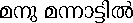
\includegraphics[scale=0.92]{name-ml}}\hspace{.1ex},
and in Hindi: \hspace{-.4ex}\raisebox{-0.7ex}{
\includegraphics[scale=0.92]{name-hi}}\hspace{-0.15ex}.

% Education {{{1
% --------------

\section{Education}

Syracuse University, Syracuse, New York, USA; August~2017--August 2023.\\
Ph.D.~in Physics, August 2023; Dissertation: \emph{\href{https://raw.githubusercontent.com/manu-mannattil/thesis/build/thesis.pdf}{Asymptotics, Geometry, and Soft Matter}}.

Indian Institute of Technology Kanpur, Kanpur, Uttar Pradesh, India; July~2009--July~2014.\\
Integrated~M.Sc.~in Physics, February~2015.

% Bhavan's Vidya Mandir, Thrissur, Kerala; June~2007--March~2009.\\
% Indian Senior School Certificate, May 2009.

% Hari Sri Vidya Nidhi School, Thrissur, Kerala; May~2005--March~2007.\\
% Indian Certificate of Seconday Education, May 2007.

% Employment History {{{1
% -----------------------

\section{Employment History}

Postdoctoral Fellow, School of Chemistry, Tel Aviv University; October 2023--.

Postdoctoral Fellow, School of Physics and Astronomy, Tel Aviv University; October 2023--.

Research Assistant, Department of Physics, Syracuse University; May 2019--August 2023.

Teaching Assistant, Department of Physics, Syracuse University; August~2017--May 2022.

Project Associate, Department of Physics, Indian Institute of Technology Kanpur;\\ September 2014--October 2015.

% Publications {{{1
% -----------------

\section{Publications}

\subsection{Works in progress}

\begin{flexlabelled}{hfill}{1.5em}{*}{*}{2.5em}{*}
  \setlength{\itemsep}{-0.25em}
  \item[1.] {\bname}, ``Energy and free-energy landscapes of soft few-body systems with singular constraints'', forthcoming.
\end{flexlabelled}

%\subsection{Preprints}

%\begin{flexlabelled}{hfill}{1.5em}{*}{*}{2.5em}{*}
% \setlength{\itemsep}{-0.25em}
% \end{flexlabelled}

\subsection{Papers}

\begin{enumerate}
  \item[7.] {\bname}, Haim Diamant, and David Andelman, ``Theory of Phase Separation in Elastomers'', \arxiv{2412.05910}{cond-mat.soft} (2024).
  \item[6.] {\bname} and Christian D.~Santangelo, ``Geometric localization of waves on thin elastic structures'', \doi{10.1103/PhysRevE.109.035001}{Phys.~Rev.~E \textbf{109}, 035001 (2024)}, \arxiv{2306.07213}{cond-mat.soft}.
  \item[5.] \bname, J.~M.~Schwarz, and Christian D.~Santangelo, ``Thermal Fluctuations of Singular Bar-Joint Mechanisms'', \doi{10.1103/PhysRevLett.128.208005}{Phys.~Rev.~Lett.~\textbf{128}, 208005 (2022)}, \arxiv{2112.04279}{cond-mat.soft}.
  \item[4.] \bname, Ambrish Pandey, Mahendra K.~Verma, and Sagar Chakraborty, ``On the applicability of low-dimensional models for convective flow reversals at extreme Prandtl numbers'', \doi{10.1140/epjb/e2017-80391-1}{Eur.~Phys.~J.~B~\textbf{90}, 259~(2017)}, \arxiv{1711.01510}{physics.flu-dyn}.
  \item[3.] \bname, Himanshu Gupta, and Sagar Chakraborty, ``Revisiting Evidence of Chaos in X-ray Light Curves: The Case of GRS~1915+105'', \doi{10.3847/1538-4357/833/2/208}{Astrophys.~J.~\textbf{833}, 208~(2016)}, \arxiv{1611.02264}{astro-ph.HE}.
  \item[2.] Aditya Tandon, Malte Schr\"{o}der, \bname, Marc Timme, and Sagar Chakraborty, ``Synchronizing noisy nonidentical oscillators by transient uncoupling'', \doi{10.1063/1.4959141}{Chaos \textbf{26}, 094817~(2016)}, \arxiv{1611.02298}{nlin.CD}.
  \item[1.] Malte Schr\"{o}der, \bname, Debabrata Dutta, Sagar Chakraborty, and Marc Timme, ``Transient Uncoupling Induces Synchronization'', \doi{10.1103/PhysRevLett.115.054101}{Phys.~Rev.~Lett.~\textbf{115}, 054101~(2015)}, \arxiv{1508.06545}{nlin.CD}.
\end{enumerate}

\subsection{Scientific software}

\begin{enumerate}
  \item[1.] \href{https://github.com/manu-mannattil/NoLiTSA}{NoLiTSA} is a Python module for nonlinear time series analysis that I developed between 2015 and 2017.  It has now been used in over 15 scientific publications, and has over 100 stars on GitHub.
\end{enumerate}

% Awards and Honors {{{1
% ----------------------

\section{Awards and Honors}

Bloomfield Postdoctoral Fellowship, Tel Aviv University, October 2023.

College of Arts \& Sciences Award, Syracuse University, May 2020.

Henry Levinstein Fellowship, Department of Physics, Syracuse University, April 2018.

Kishore Vaigyanik Protsahan Yojana, Department of Science and Technology, Government of India, March 2011.

% Talks {{{1
% ----------

\section{Talks and Posters}

Geometric Localization of Waves on Thin Elastic Structures: Tel Aviv University, February 2024; The Technion -- Israel Institute of Technology, August 2024.

A Linear Model for Elastic Phase Separation: BioSoft Day, Tel Aviv University, June 2024.

Asymptotics, Geometry, and Soft Matter: Tel Aviv University, March 2023; Georgia Institute of Technology, March 2023; Universit\'{e} Paris-Saclay, March 2023.

Can One Hear the Shape of a Filament?: APS March Meeting '23, Las Vegas.

Thermal Fluctuations of Singular Bar-Joint Mechanisms: APS March Meeting '22, Chicago; Simons Center for Geometry and Physics, Stony Brook University, May 2022.

Thermal Fluctuations of Singular Networks: APS March Meeting '21, Virtual.

Topics in Nonlinear Time Series Analysis: Indian Institute of Technology Kanpur, August 2015.

% Service {{{1
% ------------

\nohangpars

\section{Service to Profession}

Manuscript reviewer for \emph{Physics of Fluids}.

% Teaching {{{1
% -------------

\section{Teaching Experience}

\subsection{Syracuse University}

%Instructor for PHY 212 (Electricity \& Magnetism); Grader for PHY 731 (Graduate Statistical Mechanics); Teaching Assistant for PHY 215 (Honors Mechanics), PHY 211 (General Mechanics), PHY 222 (Electricity \& Magnetism Lab), and AST 101 (Introductory Astronomy).

\begin{tabular}{@{}lr}
  Grader, PHY 741: Graduate Statistical Mechanics                                              & \emph{Spring 2022} \\
  Teaching Assistant, PHY 212: General Physics II (Electricity \& Magnetism)                   & \emph{Spring 2020} \\
  Teaching Assistant, AST 101: Our Corner of the Universe                                      & \emph{Fall 2019}   \\
  Course Instructor, PHY 212: General Physics II (Electricity \& Magnetism)                    & \emph{Summer 2019} \\
  Teaching Assistant, PHY 222: General Physics II Lab (Electricity \& Magnetism)               & \emph{Spring 2019} \\
  Teaching Assistant, PHY 211: General Physics I (Mechanics)                                   & \emph{Fall 2018}   \\
  Teaching Assistant, PHY 215: General Physics I for Majors (Mechanics)                        & \emph{Fall 2018}   \\
  Teaching Assistant, AST 101: Our Corner in the Universe                                      & \emph{Summer 2018} \\
  Teaching Assistant, PHY 212: General Physics II (Electricity \& Magnetism)                   & \emph{Spring 2018} \\
  Teaching Assistant, AST 101: Our Corner in the Universe                                      & \emph{Fall 2017}
\end{tabular}

% Miscellaneous {{{1
% ------------------

\section{Miscellaneous}

\hangpars

\emph{Languages.\enspace} English (fluent), Hindi (basic), and Malayalam (native).

\emph{Computer skills.\enspace} Experience writing well-documented and modular software in Python, C++, Mathematica, Vim script, AWK, and various shells (Bash, POSIX sh, etc.); seasoned user of Unix-like operating systems and related software.

% References {{{1
% ---------------

\section{References}

\phantom{}\\[-2em]

\begin{minipage}[t]{0.28\textwidth}
  \begin{tabular}{@{}l}
  Christian D.~Santangelo\\
  Department of Physics\\
  Syracuse University\\
  \email{cdsantan@syr.edu}
  \end{tabular}
\end{minipage}
%
\begin{minipage}[t]{0.28\textwidth}
  \begin{tabular}{@{}l}
  David Andelman\\
  School of Physics\\
  Tel Aviv University\\
  \email{andelman@post.tau.ac.il}
  \end{tabular}
\end{minipage}
%
\begin{minipage}[t]{0.28\textwidth}
  \begin{tabular}{@{}l}
  Haim Diamant\\
  School of Chemistry\\
  Tel Aviv University\\
  \email{hdiamant@tauex.tau.ac.il}
  \end{tabular}
\end{minipage}

%\phantom{}\\[-0.5em]

%\begin{minipage}[t]{0.28\textwidth}
%  \begin{tabular}{@{}l}
%  Jennifer M.~Schwarz\\
%  Department of Physics\\
%  Syracuse University\\
%  \email{jmschwa02@syr.edu}
%  \end{tabular}
%\end{minipage}
%%
%\begin{minipage}[t]{0.28\textwidth}
%  \begin{tabular}{@{}l}
%  Sagar Chakraborty\\
%  Department of Physics\\
%  Indian Insitute of Technology Kanpur\\
%  \email{sagarc@iitk.ac.in}
%  \end{tabular}
%\end{minipage}

% Revision Information {{{1
% -------------------------

\bigskip

\begin{center}
  \color{gray}
  Git commit \href{https://github.com/manu-mannattil/vitae/tree/\gitHash}{\texttt{\gitShortHash}}; \gitCommitterDate
\end{center}

\end{document}
